\begin{figure}[ht!]
        \centering                     
        \footnotesize
    \setlength\tabcolsep{2pt}
    \vspace{-0.2in}
    \begin{tabular}{cccc}
        \textbf{\bdraw-350M} & \textbf{\bdraw-750M} & \textbf{\bdraw-3B} & \textbf{\bdraw-20B} \\[2mm]

        
\includegraphics[width=0.24\textwidth]{figures/scaling_comparison/infinity_0.jpg} &
        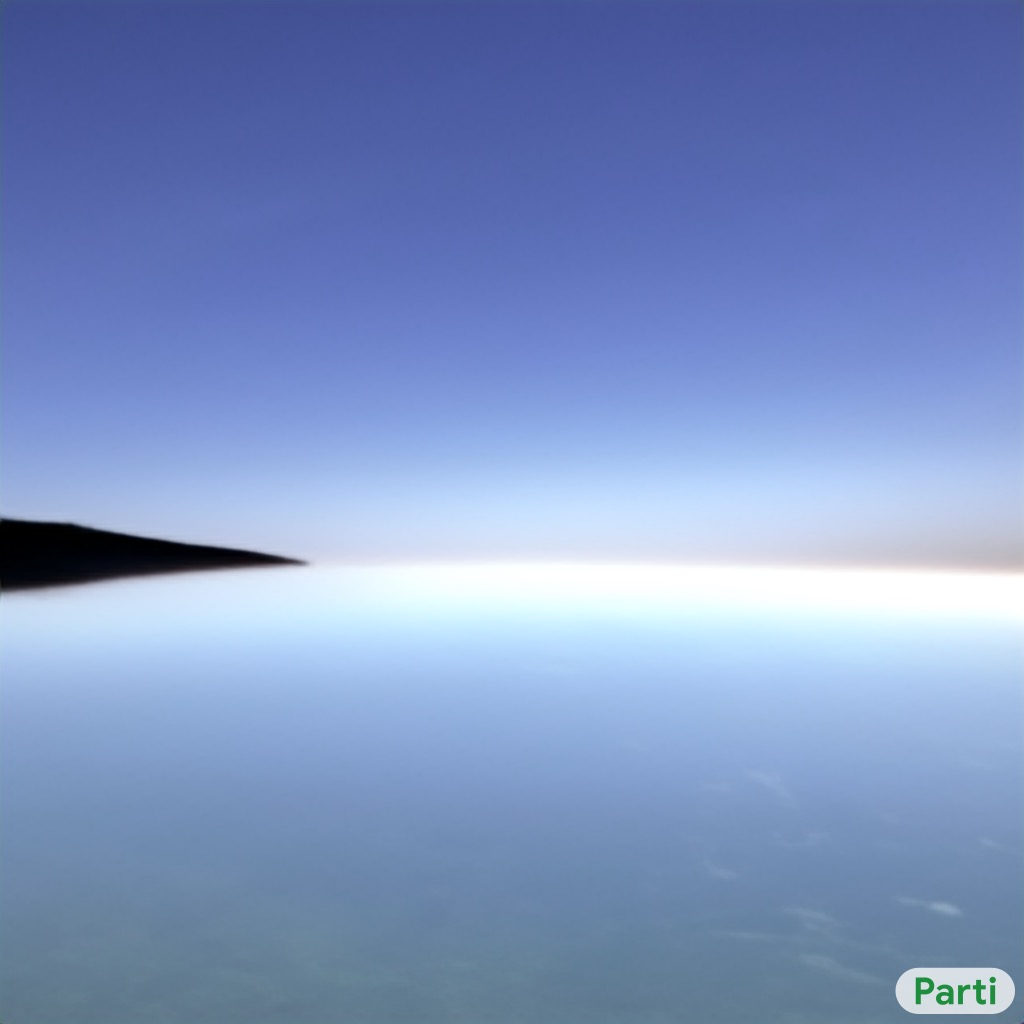
\includegraphics[width=0.24\textwidth]{figures/scaling_comparison/infinity_1.jpg} &
        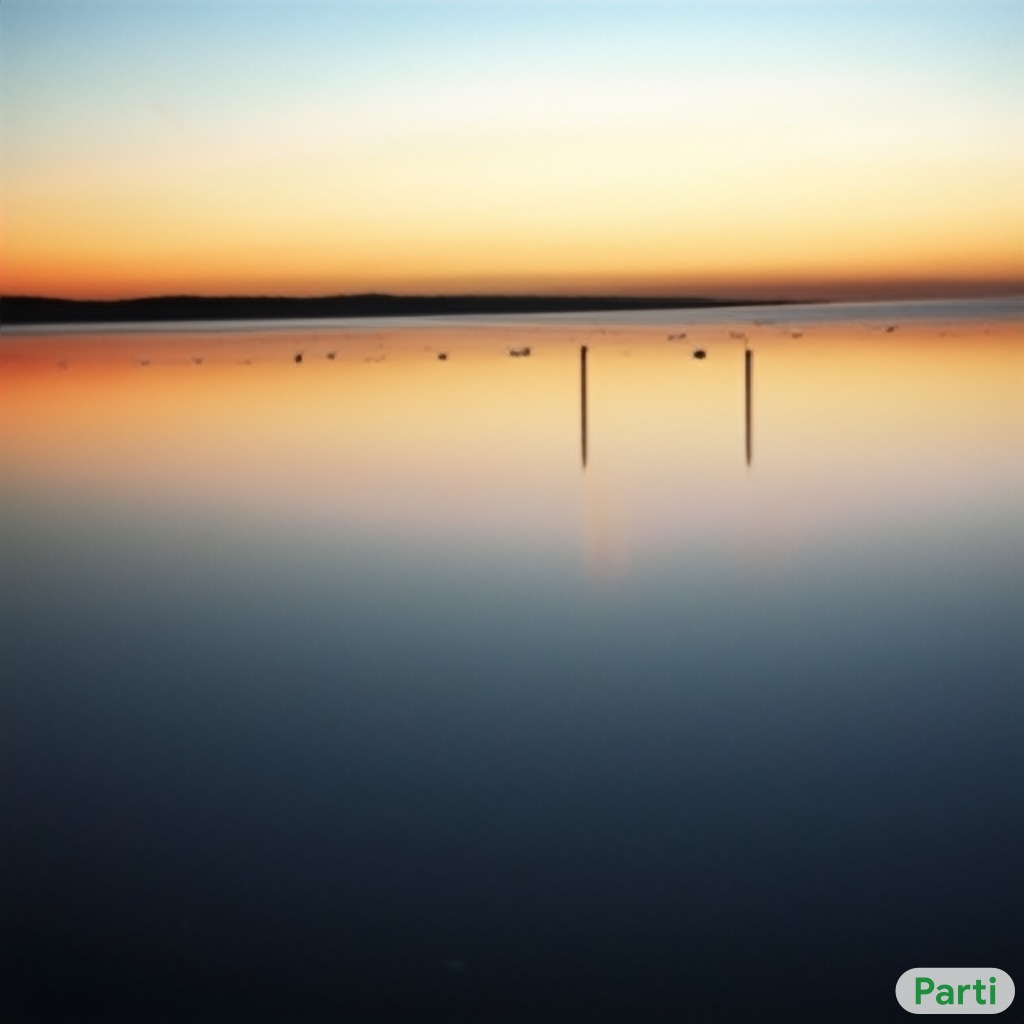
\includegraphics[width=0.24\textwidth]{figures/scaling_comparison/infinity_2.jpg} &
        
\includegraphics[width=0.24\textwidth]{figures/scaling_comparison/infinity_3.jpg}\vspace{1mm} \\
        \multicolumn{4}{c}{\small Infinity}\vspace{3mm}\\

        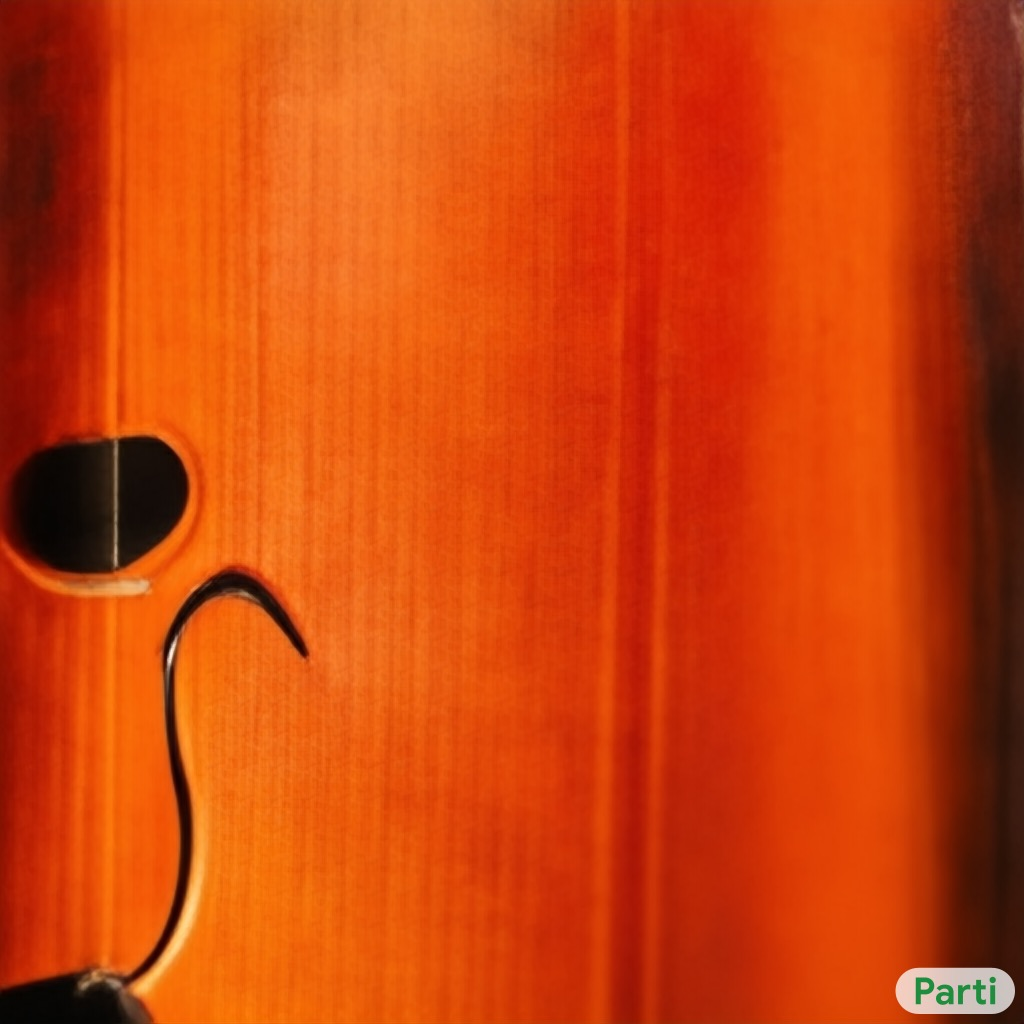
\includegraphics[width=0.24\textwidth]{figures/scaling_comparison/violin_0.jpg} &
        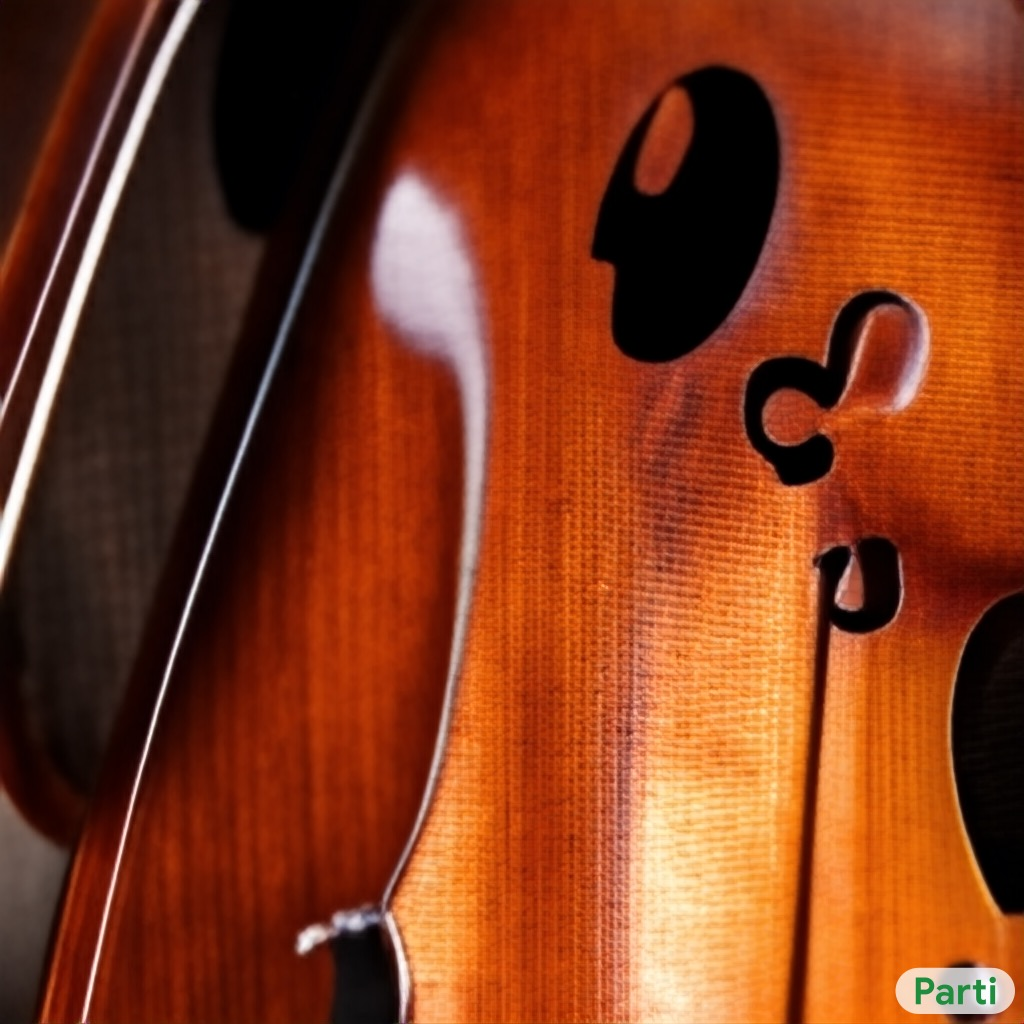
\includegraphics[width=0.24\textwidth]{figures/scaling_comparison/violin_1.jpg} &
        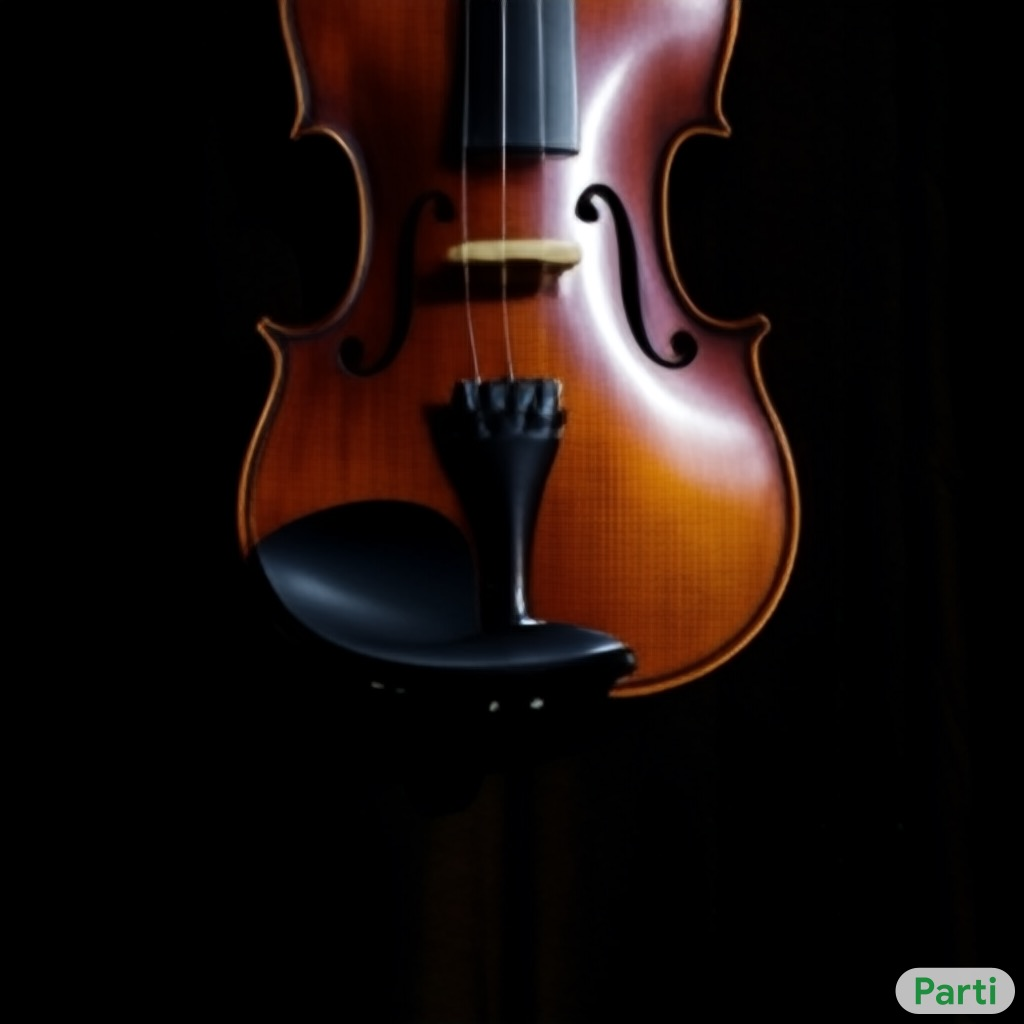
\includegraphics[width=0.24\textwidth]{figures/scaling_comparison/violin_2.jpg} &
        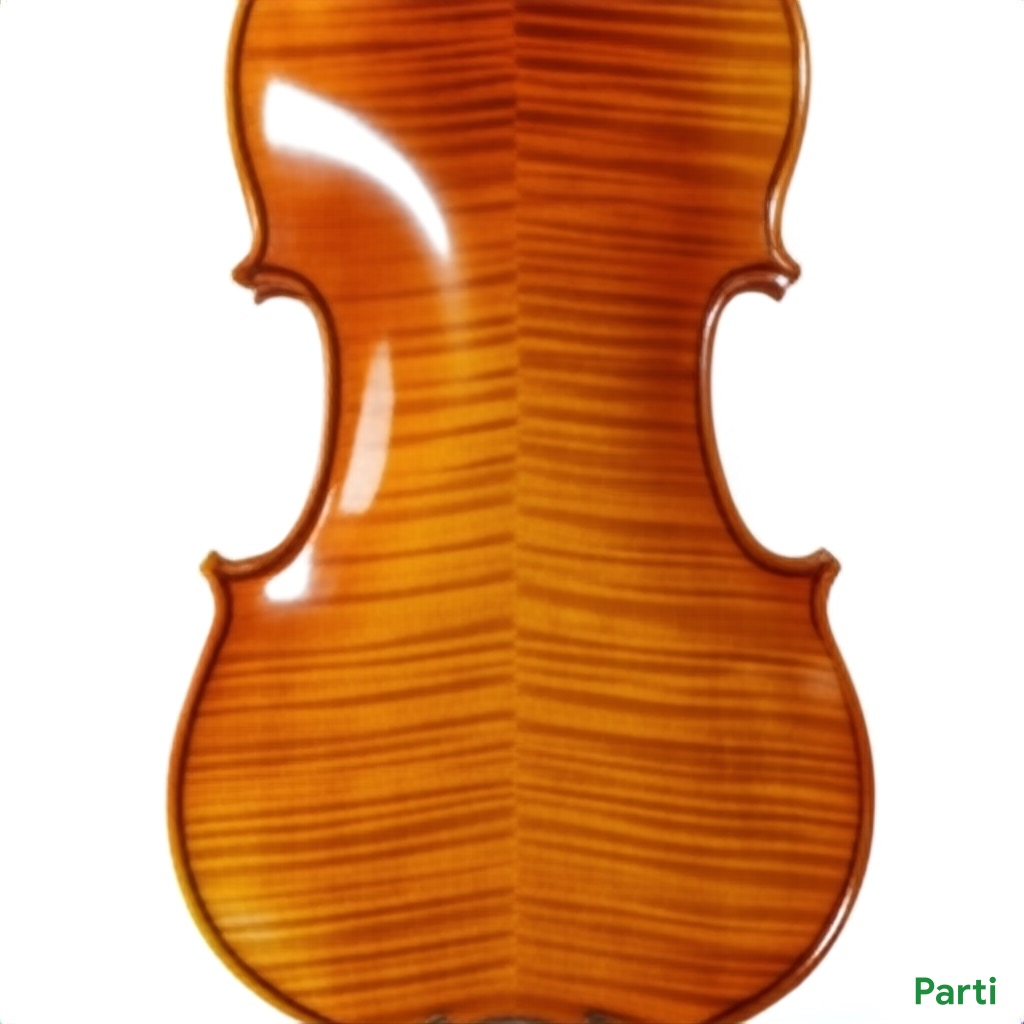
\includegraphics[width=0.24\textwidth]{figures/scaling_comparison/violin_3.jpg}\vspace{1mm} \\
        \multicolumn{4}{c}{\small The back of a violin}\vspace{3mm}\\

        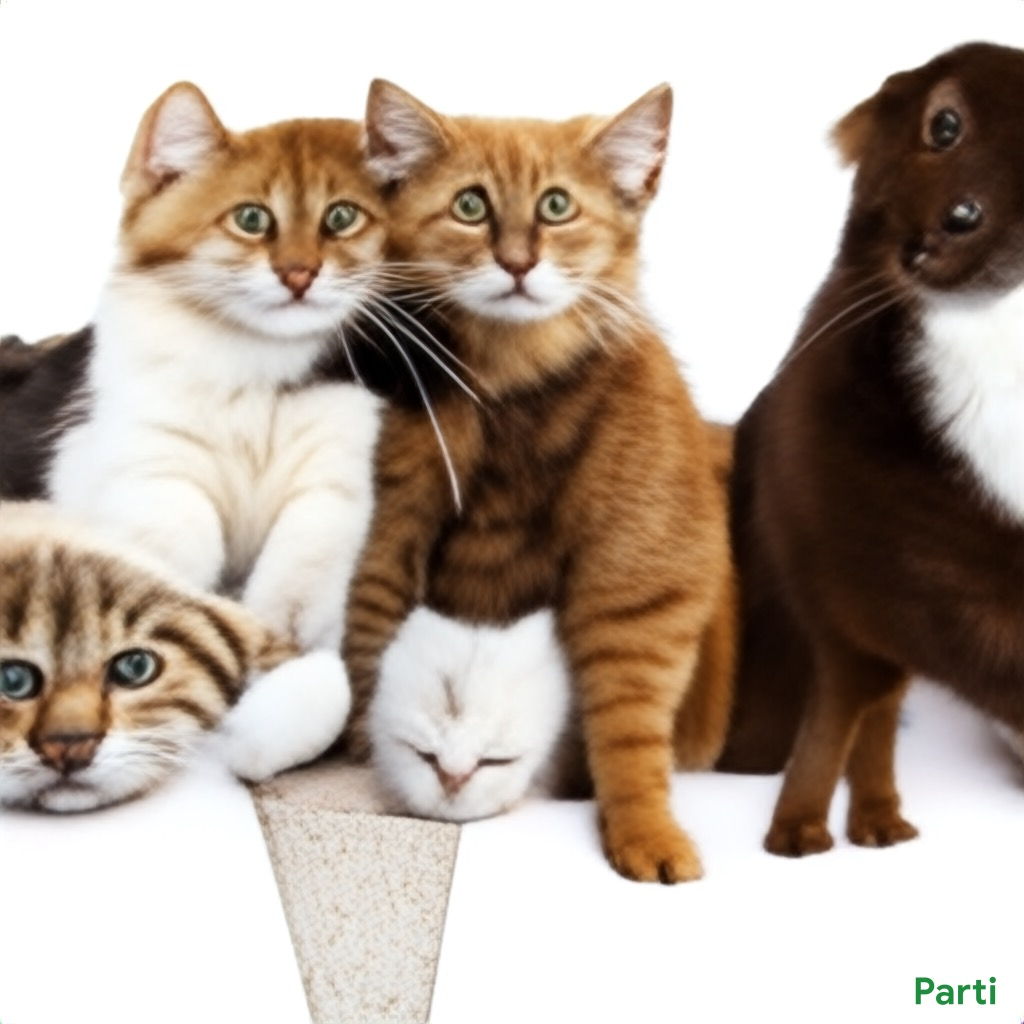
\includegraphics[width=0.24\textwidth]{figures/scaling_comparison/surrounding_0.jpg} &
        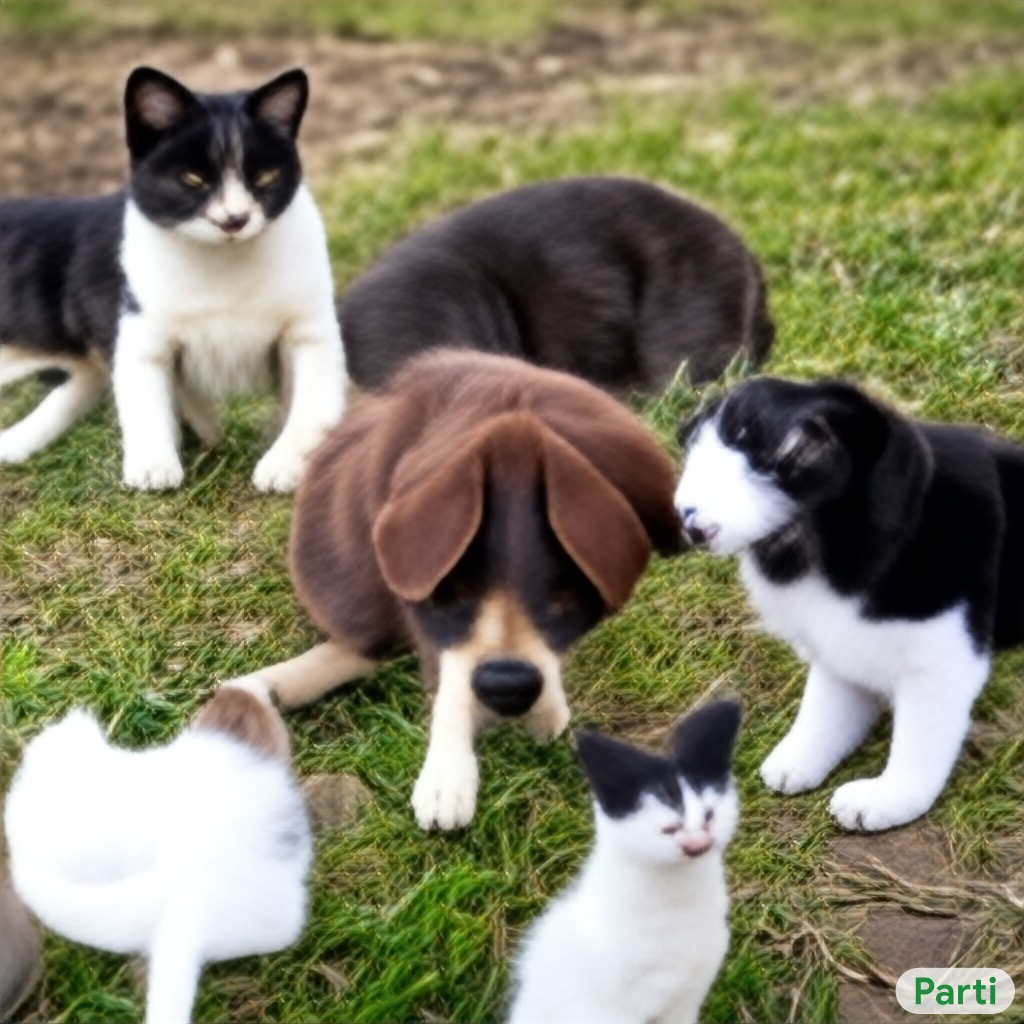
\includegraphics[width=0.24\textwidth]{figures/scaling_comparison/surrounding_1.jpg} &
        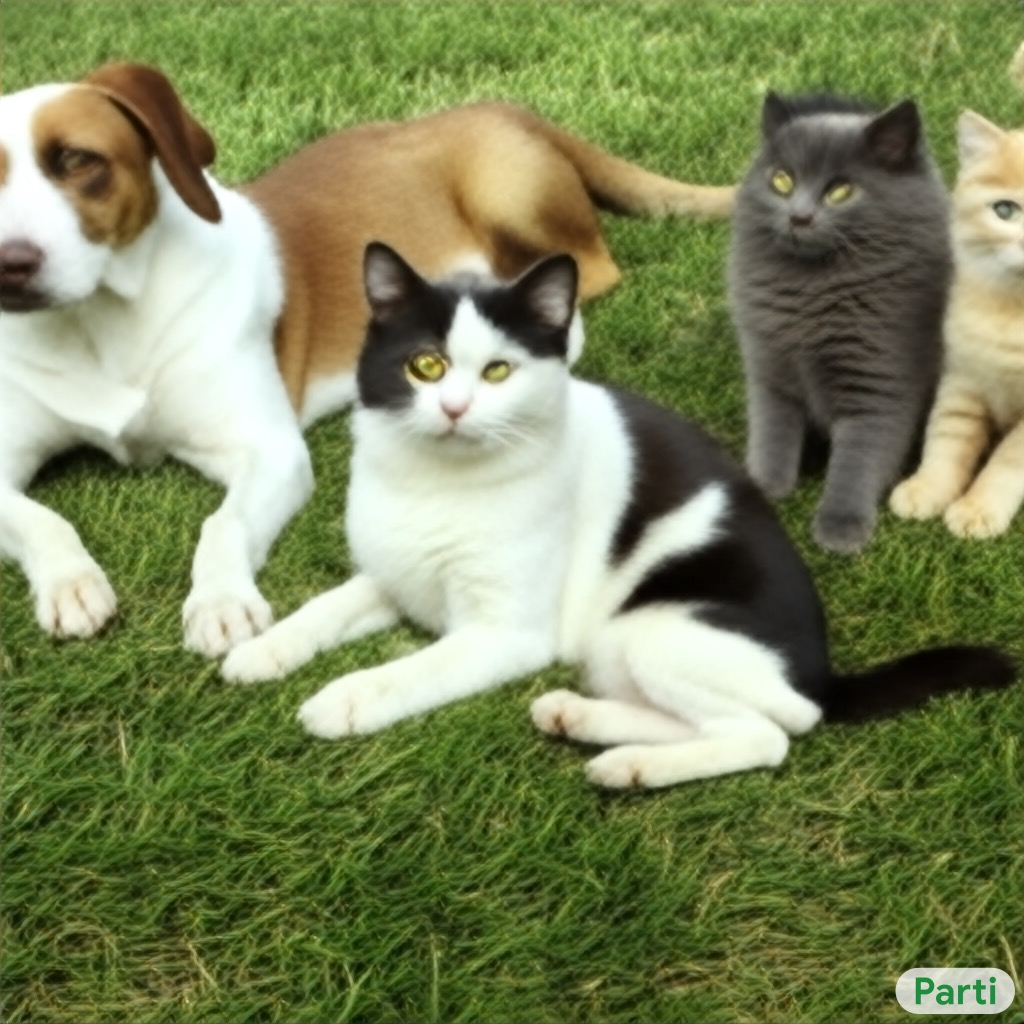
\includegraphics[width=0.24\textwidth]{figures/scaling_comparison/surrounding_2.jpg} &
        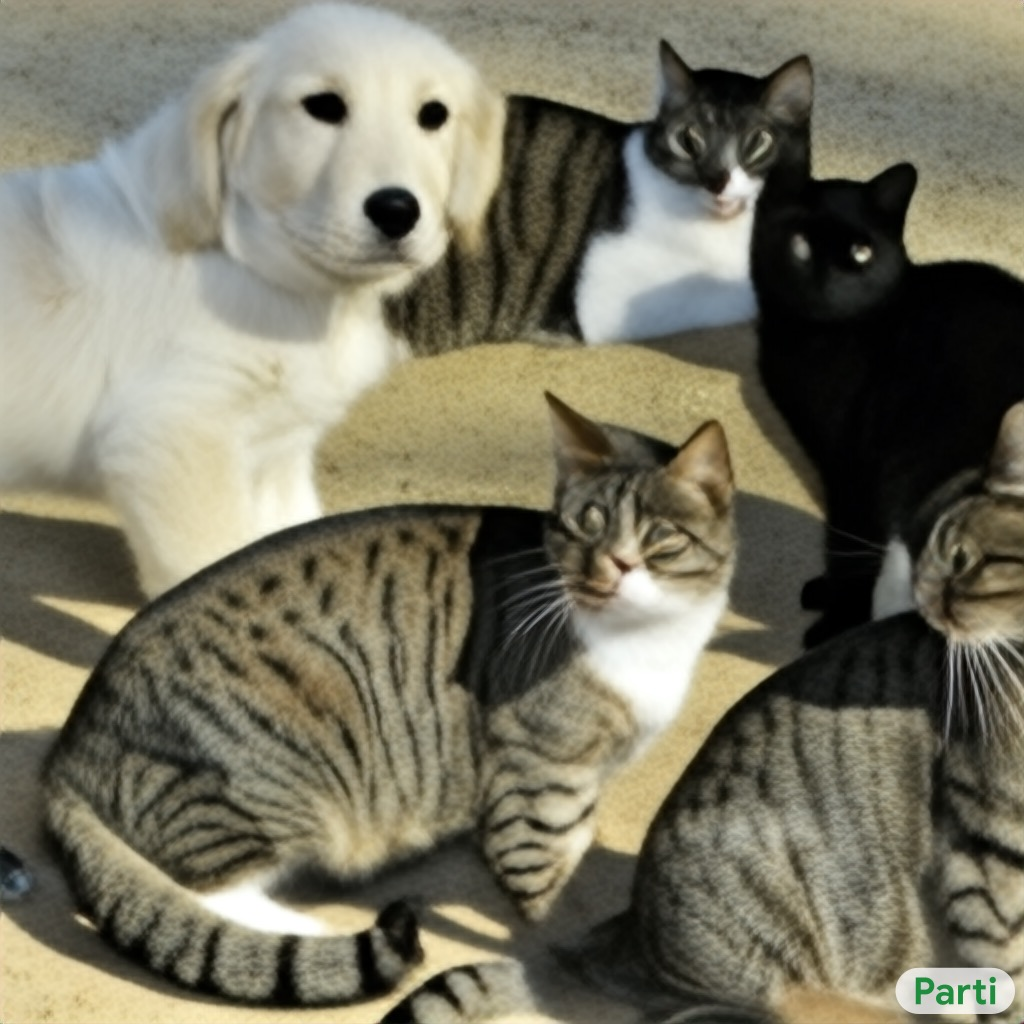
\includegraphics[width=0.24\textwidth]{figures/scaling_comparison/surrounding_3.jpg}\vspace{1mm} \\
        \multicolumn{4}{c}{\small Four cats surrounding a dog}\vspace{3mm}\\

        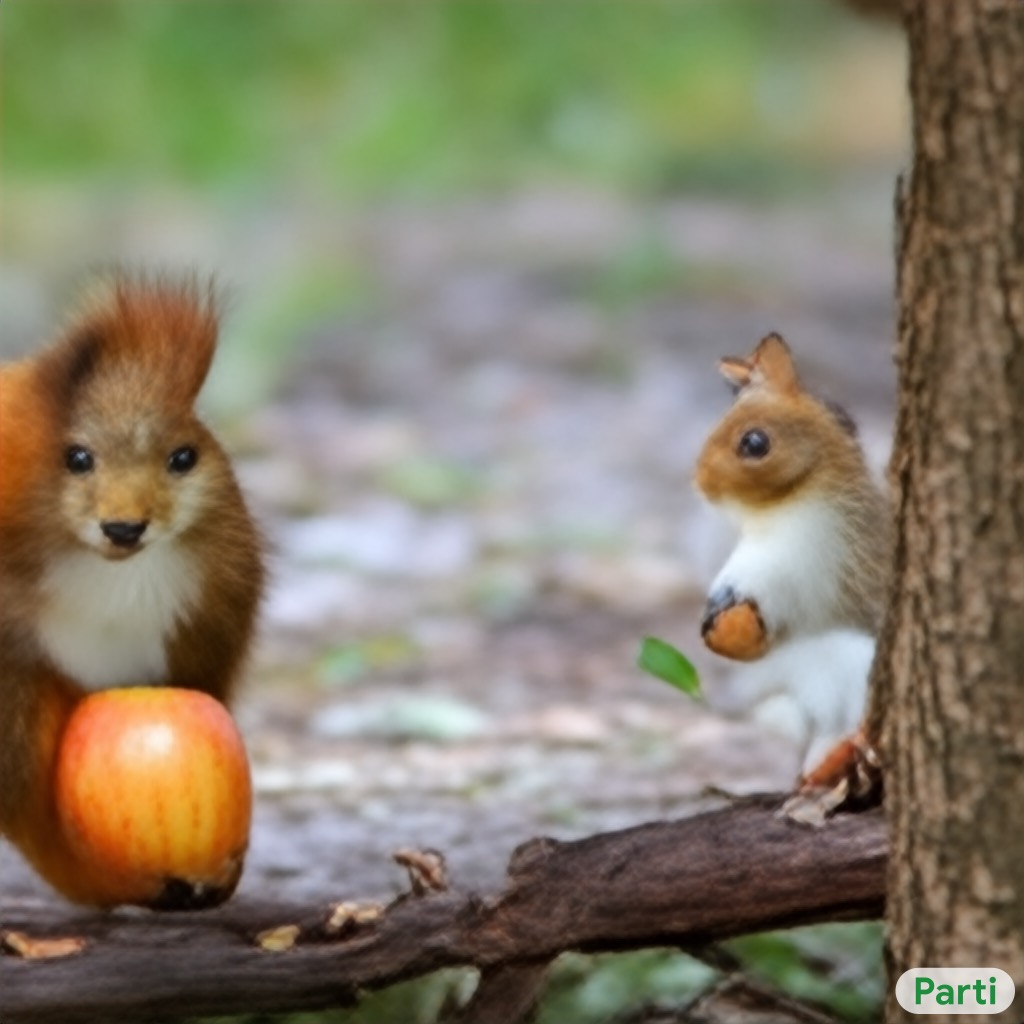
\includegraphics[width=0.24\textwidth]{figures/scaling_comparison/apple_0.jpg} &
        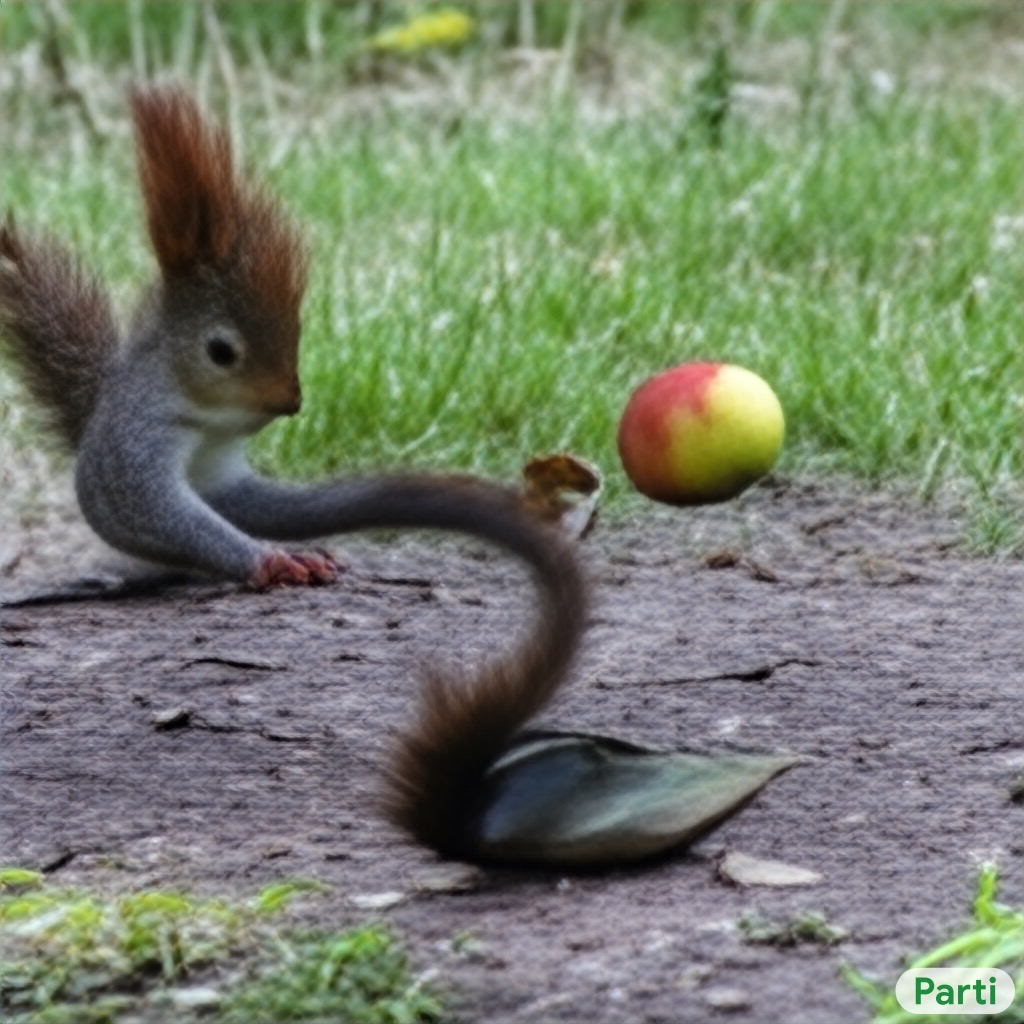
\includegraphics[width=0.24\textwidth]{figures/scaling_comparison/apple_1.jpg} &
        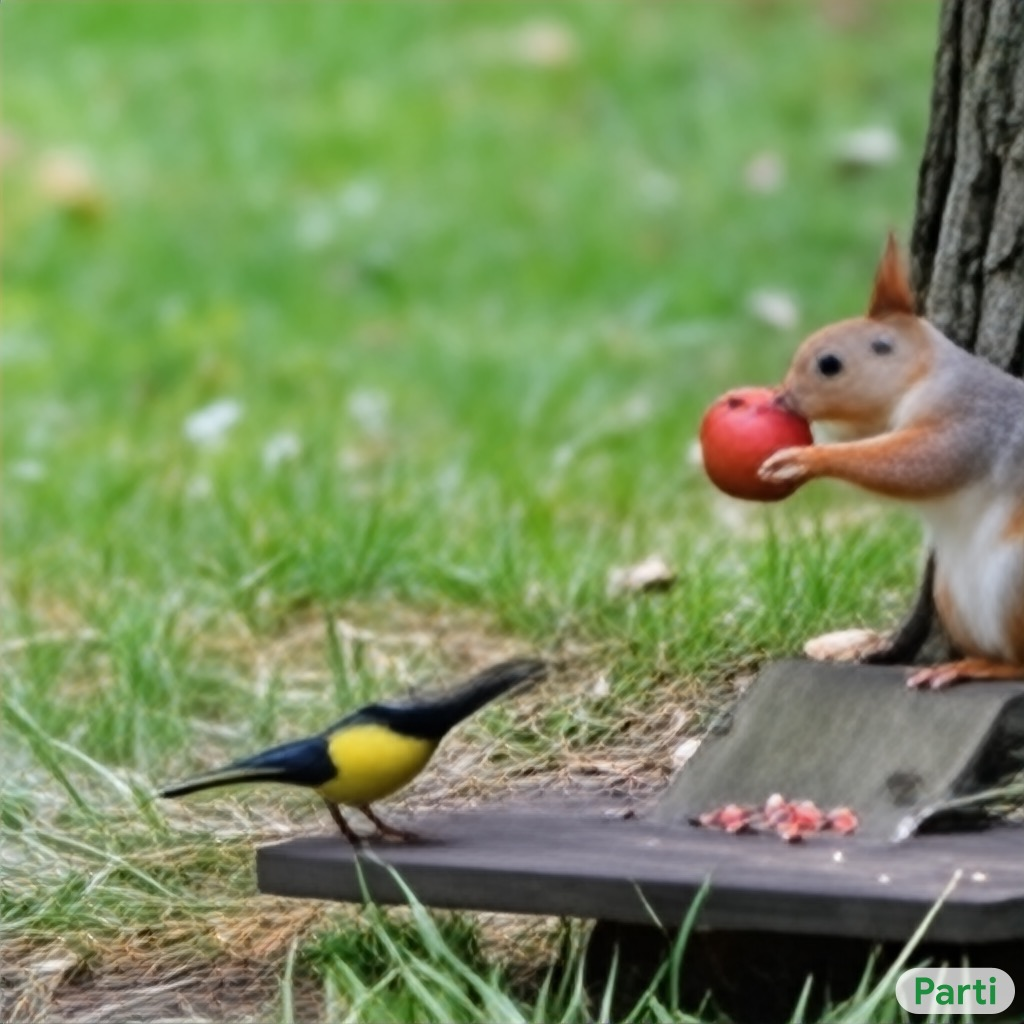
\includegraphics[width=0.24\textwidth]{figures/scaling_comparison/apple_2.jpg} &
        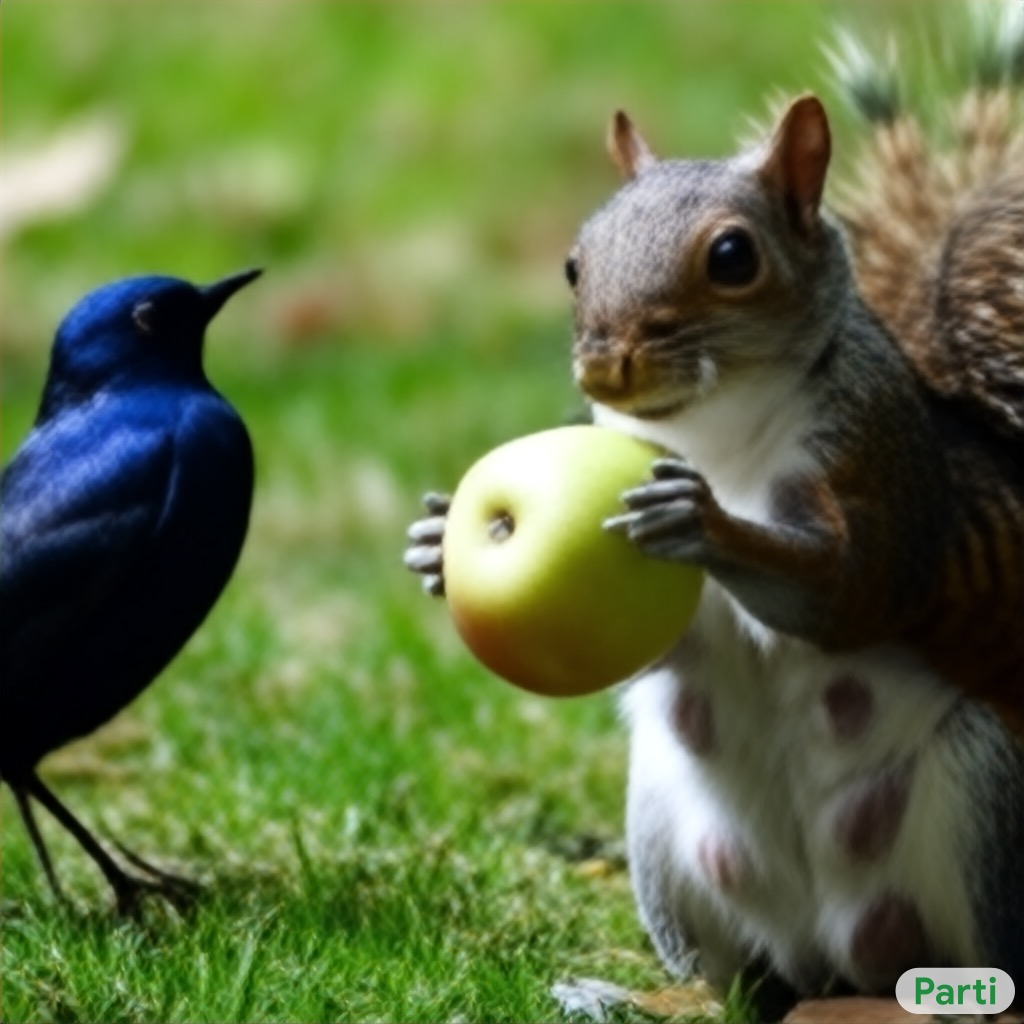
\includegraphics[width=0.24\textwidth]{figures/scaling_comparison/apple_3.jpg}\vspace{1mm} \\
        \multicolumn{4}{c}{\small A squirrel gives an apple to a bird}\vspace{3mm}\\

        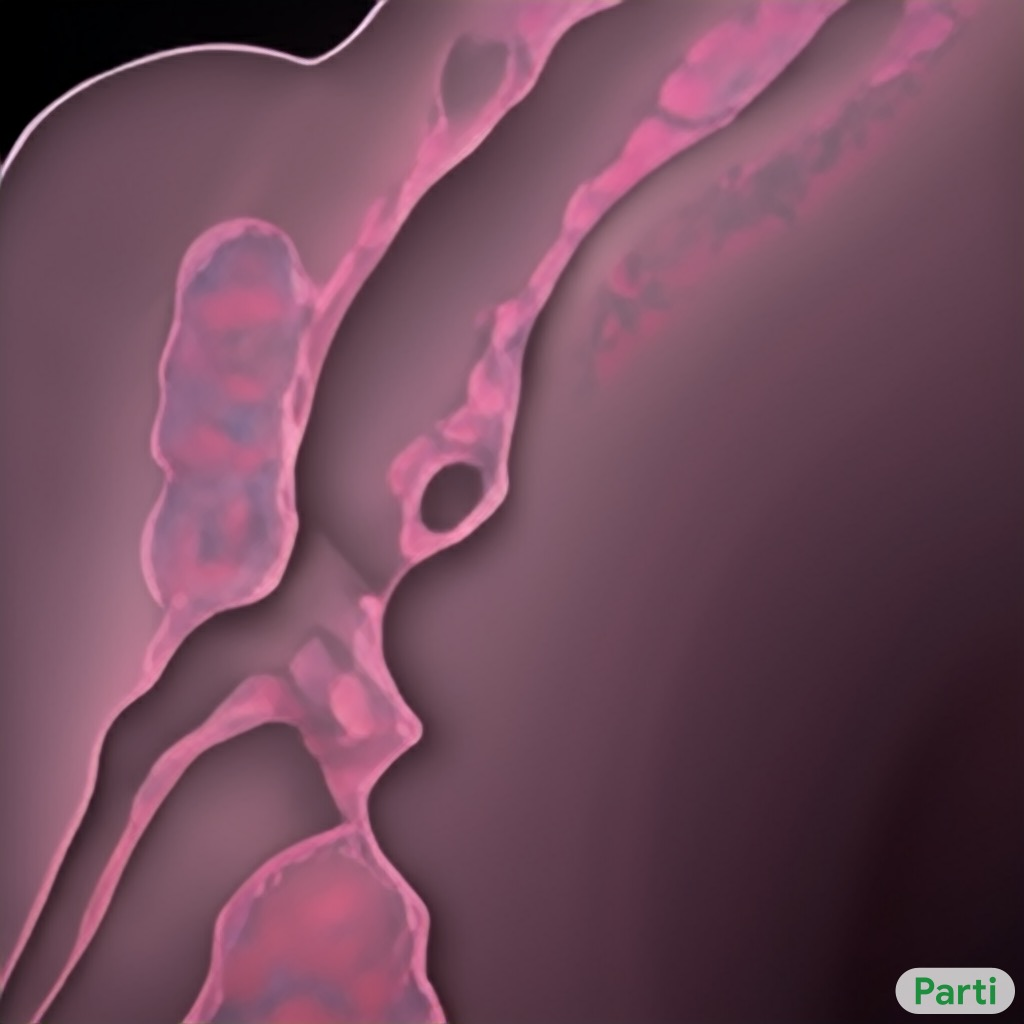
\includegraphics[width=0.24\textwidth]{figures/scaling_comparison/med_0.jpg} &
        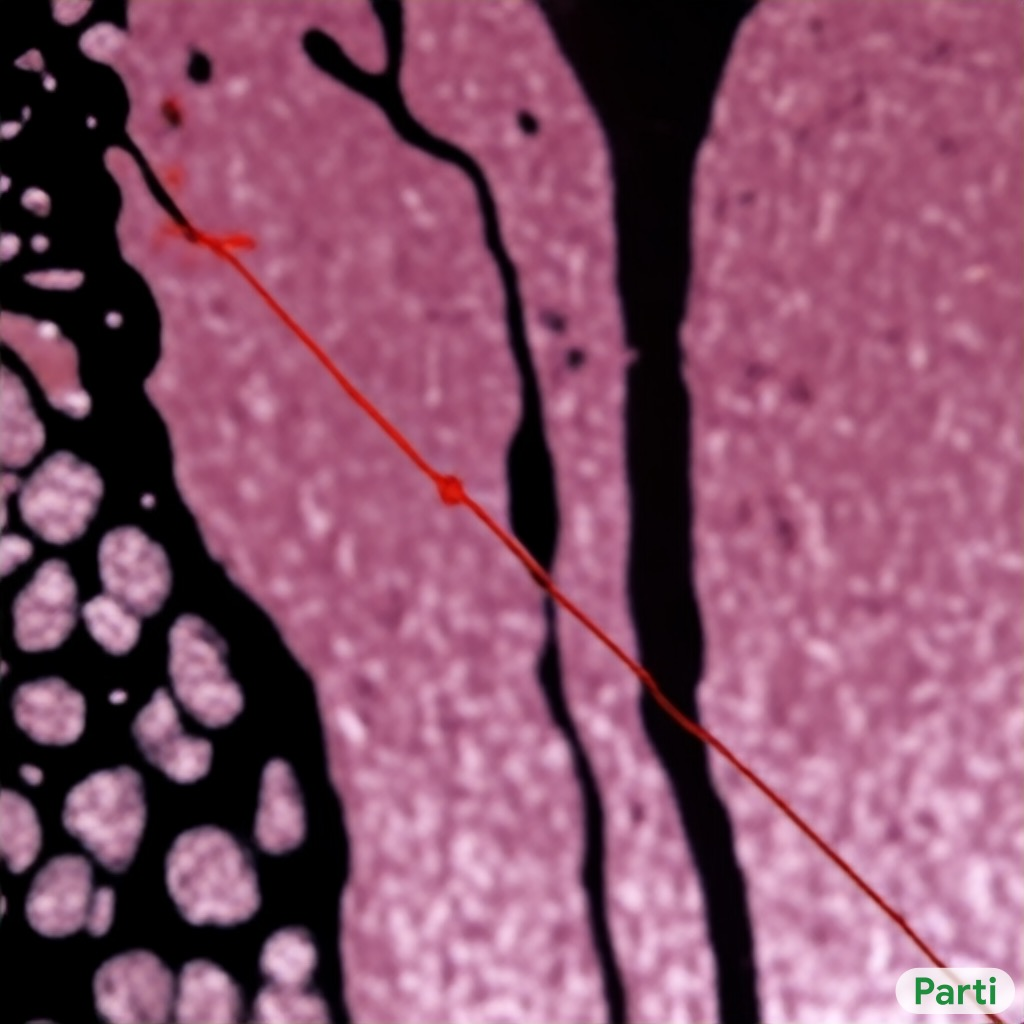
\includegraphics[width=0.24\textwidth]{figures/scaling_comparison/med_1.jpg} &
        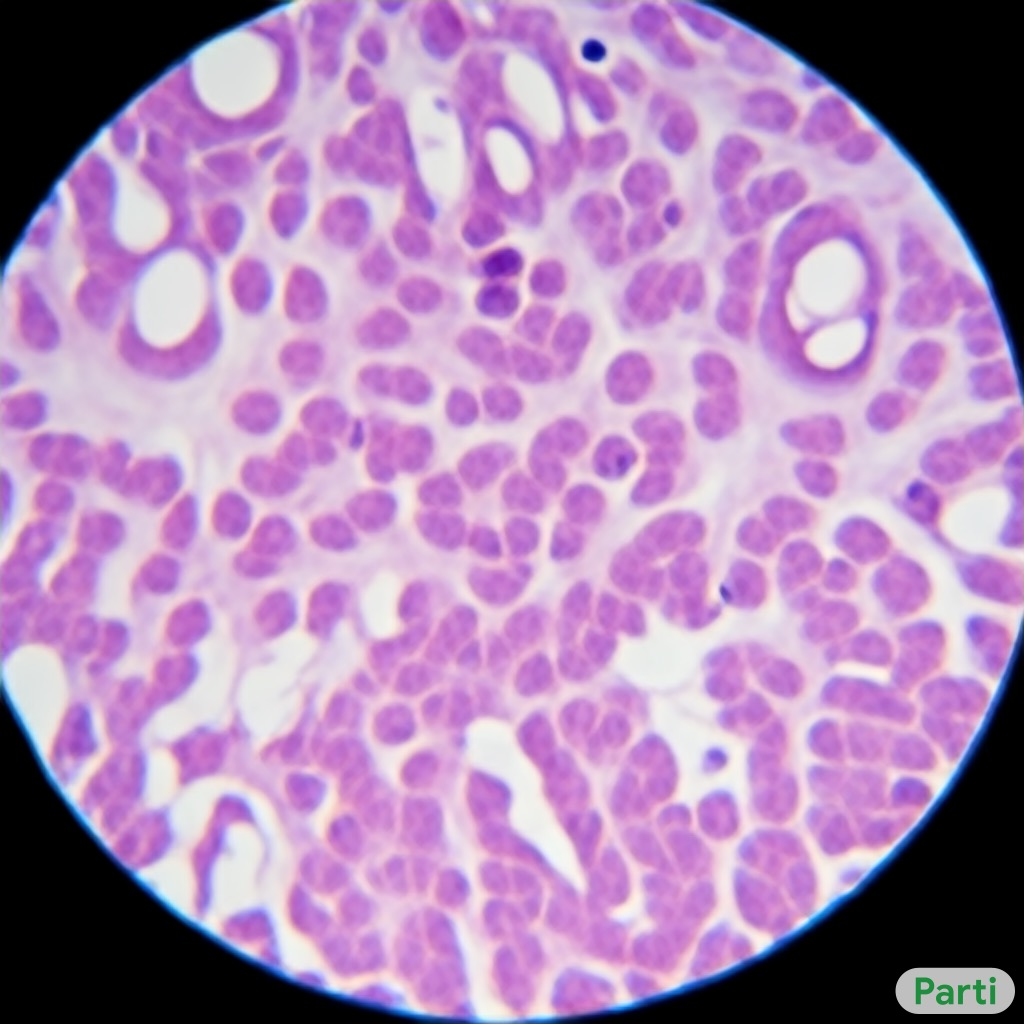
\includegraphics[width=0.24\textwidth]{figures/scaling_comparison/med_2.jpg} &
        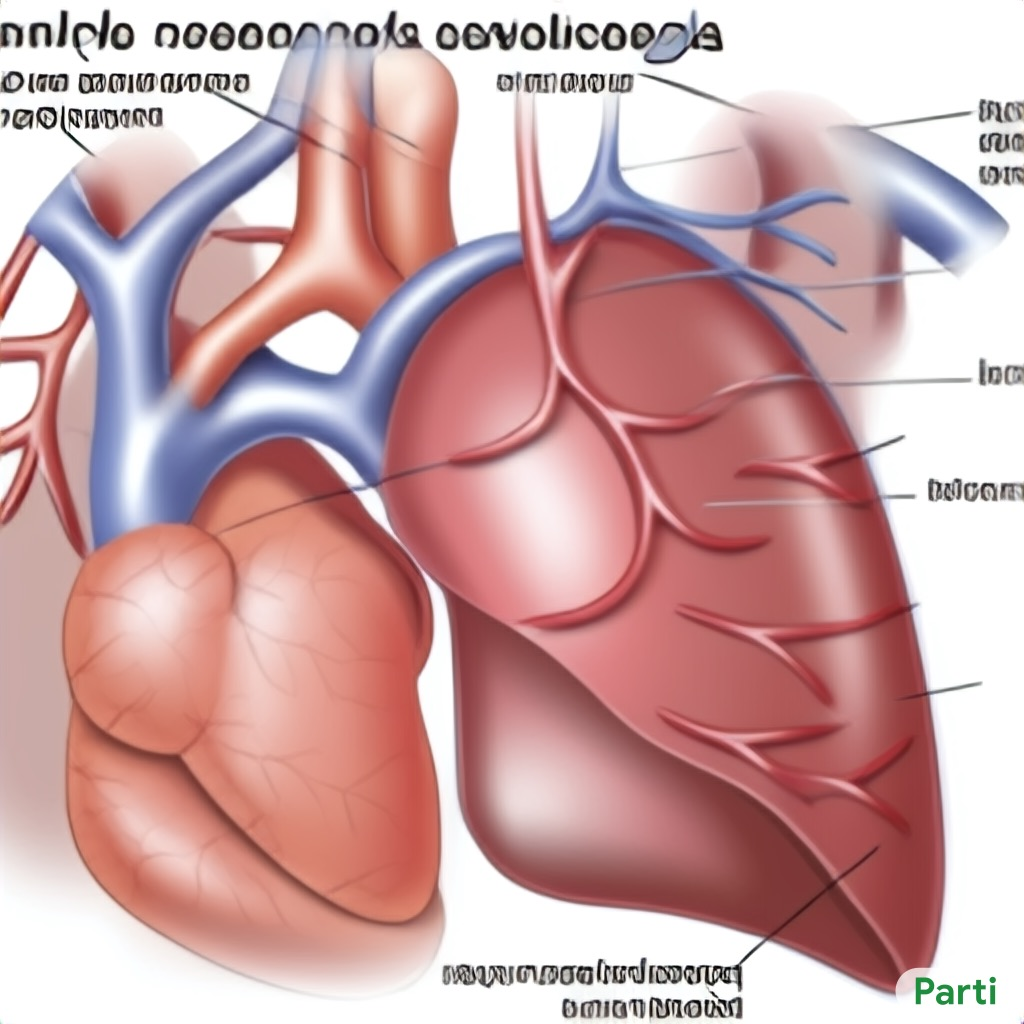
\includegraphics[width=0.24\textwidth]{figures/scaling_comparison/med_3.jpg}\vspace{1mm} \\
        \multicolumn{4}{c}{\small Pneumonoultramicroscopicsilicovolcanoconiosis} \\
    \end{tabular} 
    \caption{Qualitative comparison of scaling \bdraw models, similar to Figure~\ref{figs:scaling_comparison}. We show that simple prompts from the \bcpa{} benchmark (Section~\ref{secs:bcp}) can also be quite challenging. These examples test concepts such as \bcpstyle{Abstract}, \bcpstyle{Perspective}, \bcpstyle{Quantity}, and \bcpstyle{Linguistic Structure}.}
    \vspace{-0.15in}
    \label{figs:scaling_bcp}
\end{figure}